\documentclass{standalone}
\usepackage{tikz}

\begin{document}
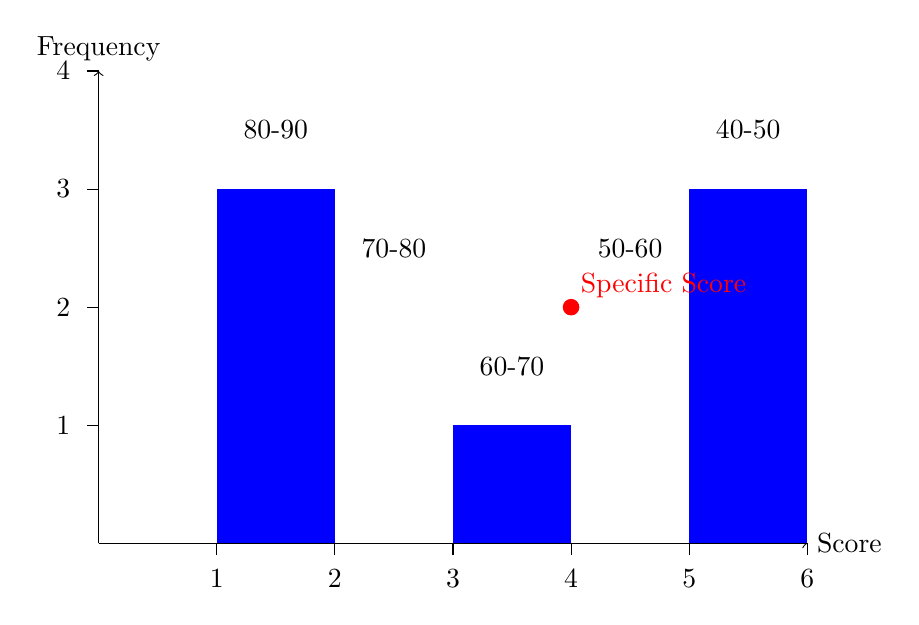
\begin{tikzpicture}[scale=1.5]
    % Axis setup
    \draw[->] (0,0) -- (6,0) node[right] {Score};
    \draw[->] (0,0) -- (0,4) node[above] {Frequency};

    % Draw the histogram bars
    \fill[blue] (1,0) rectangle (2,3);
    \fill[white] (2,0) rectangle (3,2);
    \fill[blue] (3,0) rectangle (4,1);
    \fill[white] (4,0) rectangle (5,2);
    \fill[blue] (5,0) rectangle (6,3);

    % Red dot at a specific score
    \fill[red] (4,2) circle (2pt) node[anchor=south west] {Specific Score};

    % Labels for each bar
    \node at (1.5,3.5) {80-90};
    \node at (2.5,2.5) {70-80};
    \node at (3.5,1.5) {60-70};
    \node at (4.5,2.5) {50-60};
    \node at (5.5,3.5) {40-50};

    % X-axis tick marks and labels
    \foreach \x in {1,2,3,4,5,6} {
        \draw (\x,0) -- ++(0,-0.1);
        \node at (\x,-0.3) {\x};
    }

    % Y-axis tick marks and labels
    \foreach \y in {1,2,3,4} {
        \draw (0,\y) -- ++(-0.1,0);
        \node at (-0.3,\y) {\y};
    }
\end{tikzpicture}
\end{document}